In this section, the layer is described in some detail in terms of its specific subsystems. Describe each of the layers and its subsystems in a separate chapter/major subsection of this document. The content of each subsystem description should be similar. Include in this section any special considerations and/or trade-offs considered for the approach you have chosen.

\subsection{Secondary Processing Subsystem}
The secondary processing subsystem is responsible for activation of the secondary sensors and detection system after the object is suspected to be a drone.

\begin{figure}[h!]
	\centering
 	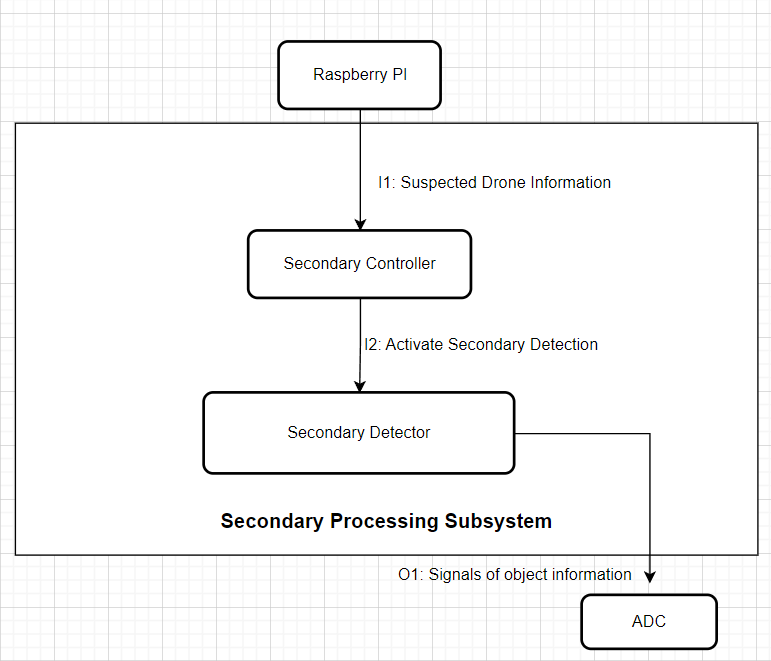
\includegraphics[width=0.60\textwidth]{images/Secondary Processing_Subsystem.png}
 \caption{Secondary Processing Subsystem}
\end{figure}

\subsubsection{Assumptions}
This subsystem assumes that it has an object that is potentially a drone and this information is given by the raspberry pi. 

\subsubsection{Responsibilities}
The primary responsibility of this subsystem is to confirm that the object is a drone. It activates the secondary detection sensors which sends the signals to ADC and these signals are sent through ODAS algorithm to the raspberry pi.

\subsubsection{Subsystem Interfaces}

\begin {table}[H]
\caption {Subsystem interfaces} 
\begin{center}
    \begin{tabular}{ | p{1cm} | p{6cm} | p{3cm} | p{3cm} |}
    \hline
    ID & Description & Inputs & Outputs \\ \hline
    \#I1 & Secondary Controller & \pbox{3cm}{Drone Information} & \pbox{3cm}{Signal to secondary detector}  \\ \hline
    \#I2 & Secondary detector & \pbox{3cm}{Activate secondary sensor} & \pbox{3cm}{N/A}  \\ \hline
    \end{tabular}
\end{center}
\end{table}

\subsection{Subsystem 2}
Repeat for each subsystem

\subsection{Subsystem 3}
Repeat for each subsystem

